\documentclass{article}

%\usepackage{corl_2020} % Use this for the initial submission.
\usepackage{amsmath, amssymb}
\usepackage{amsmath,algorithm,algcompatible, multirow, graphicx, caption, subcaption}
%\usepackage[final]{corl_2020} % Uncomment for the camera-ready ``final'' version.
\usepackage[preprint]{corl_2020} % Uncomment for pre-prints (e.g., arxiv); This is like ``final'', but will remove the CORL footnote.
\usepackage{bbm}
\usepackage{algpseudocode}

\graphicspath{{Figures/}{./}}

\DeclareMathOperator*{\argmin}{argmin}
\newcommand*{\varfont}{\fontfamily{pcr}\selectfont}


\title{A Comparative Study of Asymptotically-Optimal Sampling-Based Path Planning Methods}

% The \author macro works with any number of authors. There are two
% commands used to separate the names and addresses of multiple
% authors: \And and \AND.
%
% Using \And between authors leaves it to LaTeX to determine where to
% break the lines. Using \AND forces a line break at that point. So,
% if LaTeX puts 3 of 4 authors names on the first line, and the last
% on the second line, try using \AND instead of \And before the third
% author name.

% NOTE: authors will be visible only in the camera-ready and preprint versions (i.e., when using the option 'final' or 'preprint'). 
% 	For the initial submission the authors will be anonymized.

\author{
  Jazib Ahmad \\
  Department of Computer Science \\
  University of Toronto \\
  \texttt{jazibahmad@cs.toronto.edu} \\
  %% examples of more authors
  \And
  Jimmy Woo \\
  Department of Computer Science \\
  University of Toronto \\
  \texttt{jimmywoo@cs.toronto.edu} \\
  \And
  Sumant Bagri \\
  Department of Computer Science \\
  University of Toronto \\
  \texttt{sbagri@cs.toronto.edu} \\
}


\begin{document}
\maketitle

%===============================================================================

\begin{abstract}
In this project, we perform a comparative study between three asymptotically-optimal sampling-based path planning algorithms: Fast-marching trees (FMT*), batch informed trees (BIT*), and neural rapidly random-exploring trees (NRRT*). The individual algorithms were be implemented, and their simulated performances in terms of execution time and path costs were observed on environments of various types and complexities. The performance with varying sample counts will was observed, and a qualitative comparison of the optimal paths achieved from each algorithm for a subset of the environments is provided to demonstrate how the planners handle obstacles.

Also talk about results...
\end{abstract}

% Two or three meaningful keywords should be added here
\keywords{Sampling-based planning, asymptotically optimal planning} 

%===============================================================================

\section{Introduction}
Path planning is a search problem where the goal is to find a sequence of actions that will lead to an obstacle-free optimal path from a start state to a target state. Grid-based heuristic search algorithms \cite{astar} have been proposed in the past that guarantee finding optimal paths that exists. However, these techniques do not scale well to higher dimensional problems as they require discretization of the state space. On the other hand, sampling-based path planning algorithms \cite{rrt*} can solve high-dimensional path planning problems more efficiently. However, these algorithms only converge to optimal paths asymptotically, and in practice may compute sub-optimal paths. Many attempts have been made to make improvements to sampling-based methods \cite{irrt}\cite{SBA*}\cite{RA*}, using techniques such as heuristic guided searches, or the reduction of the sampling space. In this project, we implement three sampling-based path planning algorithms, and compare their performances through simulations.

We can formulate the path planning problem by defining the state space and the cost function similar to \cite{rrt*}. Let $\mathcal{X} \in \mathbb{R}^d$, $\mathcal{X}_{free}$, and $\mathcal{X}_{obs}$ be the state space, free space, and the obstacle space respectively where $\mathcal{X}_{obs} \subset \mathcal{X}$ and $\mathcal{X}_{free}  = \mathcal{X} \setminus \mathcal{X}_{obs}$. Let $x_{init} \in \mathcal{X}_{free}$, $x_{goal} \in \mathcal{X}_{free}$ be the start and end states respectively. The goal of the path planning problem is to determine a path $\sigma$ : [0, 1] $\mapsto \mathcal{X}_{free}$ such that $\sigma(0) = x_{init}$, $\sigma(1) = \mathcal{G}(x_{goal})$, where the acceptable goal region is defined as $\mathcal{G}(x_{goal}) = \{x \, \in \, \mathcal{X} \, | \, x - x_{goal} < r\}$. Then we can define the path planning problem as minimizing the following cost function
    \begin{align}
        & \sigma^* = \argmin_{\sigma \in \Sigma} c(\sigma) \\
        & s.t. \;\, \sigma(0) = x_{init}, \; \sigma(1) = \mathcal{G}(x_{goal}), \; \sigma(t) \;  \mathcal{X}_{free}, \; \forall t \in [0,1] \nonumber
    \end{align}
    
where $\Sigma$ is the set of feasible paths and $c(\sigma)$ is the cost of a single path $\sigma$.

%===============================================================================

\section{Related Work}
\label{sec:Related Work}
    Rapidly random-exploring tree (RRT) \cite{rrt} is a well studied sampling based algorithm. It utilizes sampling to avoid the discretization of the state space and increase scalability but produces a sub-optimal path \cite{rrt*}. Many variants have been proposed to improve its performance. RRT* \cite{rrt*} optimizes the tree in each iteration, allowing the planner to converge to an optimal solution asymptotically. Informed RRT* \cite{irrt} reduces the number of iterations to convergence from RRT* by reducing the sampling space once a sub-optimal path is found. Similar work has been done to extended the Probabilistic Roadmap algorithm (PRM) as PRM* \cite{rrt*} that converges to an asymptotically optimal solution. However, these approaches do not utilize the ordered search available to grid-based planners. RA* \citep{RA*} and SBA* ~\citep{SBA*} directly extend A* to the continuous domain by sampling near heuristically selected vertices of the graph. While this is a good approach for cases with no obstacles, there is a problem of local minima for cases with obstacles. ~\citet{RA*} address this problem for RA* with a minimum allowed distance between vertices, which decreases the possible resolution of the final solution. ~\citet{SBA*} address this problem for SBA* by prioritizing sampling unexplored areas through adding a local sample density to the heuristic for selecting vertices near which to sample. The local sample density must be estimated \cite{BIT*}.
    
%===============================================================================

\section{Methodology}
\label{sec:Methodology}
We perform a comparison study of three asymptotically-optimal sampling-based path planning algorithms: Fast-marching trees (FMT*), batch informed trees (BIT*), and neural RRT (NRRT*) \cite{nrrt}. The following section briefly describe each of these algorithms.

\subsection{Fast-Marching Trees}
\label{met:fmt}
FMT* incorporates the advantages from both single and multiple query sampling-based algorithms in that it eliminates the greediness in RRT* by creating connections nearly optimally instead of trying to find the exactly optimal steering direction. However, in finding the optimal path, it grows a tree (as in the case of RRT*) instead of creating a bi-directional graph employed in the PRM* algorithm.

In the original implementation of FMT*, \citet{FMT} describe the algorithm as an outward growing tree in the cost-to-arrive space which performs a forward-dynamic programming recursion on a fixed sample size. Some of the key features of this algorithm are described below:
\begin{itemize}
	\item The sample count ($\mathcal{N}$) is fixed and the points are sampled from the free space ($\mathcal{X}_{free}$), beforehand, using a pre-determined distribution. This is described by $\mathcal{M} \subset \mathcal{X}_{free}$
	\item The tree is built by considering a subset of sampled points that are within the ball $B(\bar{x}, r_n) := \{ x \in \mathbb{R}^d: ||x - \bar{x}||_2 < r_n \}$  (i.e "disk-connected"), where $r_n$ is called the \textit{connection radius} and $\bar{x} \in \mathbb{R}^d$ is the query-point
	\item The algorithm improves in computational complexity by considering a \textit{single}, locally optimal connection, with minimum cost-to-arrive, and adds the connection to the tree only if it is collision free. If it isnt, however, then the algorithm does not try to find another \textit{"valid"} point in $B(\bar{x}, r_n)$ and simply skips the current query point $\bar{x}$
\end{itemize}

The basic pseudocode of the FMT* algorithm, as described in \cite{FMT} is described in Algorithm \ref{alg:fmt}

\begin{algorithm}
\caption{Fast Marching Tree Algorithm (FMT*): Basics}\label{alg:fmt}
	\begin{algorithmic}[1]
		\Require sample set $V$ comprising of $x_{init}$ and $n$ samples in $\mathcal{X}_{free}$, at least one of which is also $\mathcal{X}_{goal}$
		\State Place $x_{init}$ in $V_{open}$ and all other samples in $V_{unvisited}$; initialize tree with root node $x_{init}$
		\State Find lowest-cost node $z$ in $V_{open}$
		\State \quad For each of z's neighbors $x$ in $V_{unvisited}$:
		\State \quad\quad Find neighbor nodes $y$ $V_{open}$
		\State \quad\quad Find locally-optimal one-step connection to $x$ from among nodes $y$
		\State \quad\quad If that connection is collision-free, add edge to tree of paths
		\State \quad Remove successfully connected nodes $x$ from $V_{unvisited}$ and add them to $V_{open}$
		\State \quad Remove $z$ from $V_{open}$ and add it to $V_{closed}$
		\State \quad Repeat until either:
		\State \quad\quad (1) $V_{open}$ is empty $\Rightarrow$ report failure
		\State \quad\quad (2) Lowest-cost node $z$ in $V_{open}$ is in $\mathcal{X}_{goal} \Rightarrow$ return unique path to $z$ and
		\State \quad\quad\quad report success
	\end{algorithmic}
\end{algorithm}

Here, $V = \{x_{init}\} \bigcup \mathcal{M}$ and it is partitioned into three different sets: $V_{unvisited}$, $V_{open}$ and $V_{closed}$. $V_{unvisited}$ contains points that havent been explored yet. $V_{open}$ consists of query-points $\bar{x}$ whose cost-to-arrive from $x_{init}$ has been determined and are active for making new connections (i.e. tree-leaves). $V_{closed}$ consists of points which have been explored and are no-longer considered for new connections (i.e. parent nodes in the tree).

The \textit{connection radius}, $r_n$, is computed as follows (\cite{FMT}),
\begin{align}
	r_n &= \gamma \left( \frac{\log(\mathcal{N})}{\mathcal{N}} \right)^{1/d} \notag \\
	\text{where, } \gamma &> 2 \left( \frac{\mu(\mathcal{X}_{free})}{d \times \zeta_d} \right)^{1/d} \text{ and \textit{d} is the dimensionality} \notag
\end{align}

Here, $\mu(\mathcal{X}_{free})$ is the Lebesgue-measure of the free space and $\zeta_d$ is the volume of a unit-ball in d-dimensional Euclidean space

In our implementation of FMT*, we have made two notable modifications
\begin{itemize}
	\item[]\textbf{First,} We have added euclidean-heuristics (with weight$=1.0$) to the computation for cost-to-arrive at node $x$ in $V_{unvisited}$ from $x_{init}$ via a node $y$ in $V_{open}$. This is defined, mathematically, below:
	\begin{align}
		c(x) = ||x - y||_2 + 1.0 \times \left( ||x - x_{goal}||_2 - ||y - x_{goal}|| \right) \notag
	\end{align}
	\item[]\textbf{Second,} We maintain the obstacle nodes as a KDTree for faster query when checking for collisions
\end{itemize}

We define the pseudocode for performing collision checks in FMT* in Algorithm. \ref{alg:cc}
\begin{algorithm}
\caption{Algorithm for Collision Checks}\label{alg:cc}
	\begin{algorithmic}[1]
	\Require obstacles stored as a KDTree. dCol defining the collision clearance
	\State \textbf{Input: } start, target($\leftarrow \emptyset$) \Comment{check for collisions between start and target}
	\State \textbf{Output: } \textit{bool} \Comment{True if collision-free, else false}
	\Function{CollisionFree}{start, target}
		\If{target$\leftarrow \emptyset$ or start = target}
			\State \textbf{return} \Call{Near}{obstacles,start,1} $>$ dCol
		\EndIf
		\State $\overline{ts} \longleftarrow \frac{\overline{target} - \overline{start}}{||\overline{target} - \overline{start}||_2}$ \Comment{vector from start to target}
		\State pts $\longleftarrow (\overline{start}, 0.1\times\overline{ts}, \cdots, \overline{target})$ \Comment{segmenting the connecting line}
		\State \textbf{return} $\min$[\Call{Near}{obstacles,pts,1}] $>$ dCol
	\EndFunction
	\end{algorithmic}
\end{algorithm}

The performance benefits of FMT* are observed in higher dimensions (e.g. 6DoF Robotic Manipulators) where performing collision-checks is costly.

\subsection{Batch Informed Trees}
BIT* is a sampling based approach to path planning that utilizes the ordered nature of grid based approaches with the goal of creating a path planning algorithm that is both scalable and efficient. To do this, BIT* samples in batches and performs an ordered search on the batches ~\citep{BIT*}. In other words, the algorithm samples an entire batch randomly but uses a heuristic to determine which sample in the batch to process next ~\citep{BIT*}. Furthermore, similar to ~\citep{irrt}, once a sub-optimal solution is found, it reduces the region that is sampled to focus on the sub-problem that contains a better solution ~\citep{BIT*}. In this way, it maintains anytime resolution: finding a sub-optimal solution quickly, and using this sub-optimal solution to converge asymptotically towards the optimal solution ~\citep{BIT*}.

\subsection{Neural RRT*}
Neural RRT* is a non-uniform sampling-based path planning algorithm that aims to take advantage of the optimal path costs of the A* algorithm as well as the asymptotic optimality of the RRT* algorithm. Instead of sampling from the state space using just a uniform distribution, a non-uniform distribution learned by a convolutional neural network (CNN) trained on optimal paths generated from the A* algorithm is used to achieve non-uniform sampling. Unlike many of the RRT variant algorithms, the NRRT* algorithm does not depend on any human-designed heuristics to improve its performance. It also maintains the probabilistic completeness and the asymptotic optimality of the RRT* algorithm. Through simulations, it has been shown to perform superior compared to RRT* and IRRT* \cite{nrrt}.


\section{Evaluation}
\label{sec:Evaluation}

This section is structured as follows: First, we mathematically define the different path-planning metrics used in evaluation scheme. Then, we compare the performance of algorithms based on these metrics (using trend-plots generated from the simulations) to understand their behaviour in different situations. We describe a few, specific, state-space scenarios as well as some algorithmic factors and discuss their effects on the different metrics. Finally, we provide a qualitative comparison for the different paths generated by the algorithms for a specific subset of the maps and states.

\subsection{Defining the Metrics}

\subsubsection{Solution Cost ($\mathcal{J}$)}

The solution cost, $\mathcal{J}$, is defined as the cost-to-come to the goal location ({\varfont goal}) from the start location ({\varfont start}) along the path defined by the path-planning algorithm. We evaluate the cost ($\mathcal{J}$) as follows: For a set of N nodes in the free space $\mathcal{X}_{free}$, let $\mathcal{P} \subset \mathcal{X}_{free}$ be the set of nodes along the optimal path as computed by the path planning algorithm $\{ \mathcal{X}_{free}, x_{init}, \mathcal{G}(x_{goal})\}$; Then the cost $\mathcal{J}$ is defined as: 
\begin{align}
    \mathcal{J} = \sum_{i=1}^{N} ||x_i - Parent(x_i)||_2 \text{, where } x_i \in \mathcal{P}
\end{align}

\subsubsection{Execution Time ($\mathcal{T}$)}

The execution time is defined differently for BIT* and FMT*/NRRT*. For FMT* and NRRT*, the execution time is the time it takes for the algorithm to find any feasible solution from {\varfont start} to {\varfont goal}. Whereas, for BIT*, the execution time is calculated based on the maximum number of iterations the algorithm can perform before terminating.

Formally, we evaluate the exection time, $\mathcal{T}$,  as follows: Let, $\tau_{fmt}$, $\tau_{bit}$ and $\tau_{nrrt}$ denote the time-per-iteration for the FMT*, BIT* and NRRT* algorithms respectively. Let, $n_{fmt}$ and $n_{nrrt}$ denote the number of iterations performed by FMT* and NRRT*, respectively, before they find a solution. Also, we cap the maximum number of iterations that can be performed by each algorithm with a common value. Let this be $n\_max$. Then the execution time $\mathcal{T}$ is defined as:

\begin{align}
	\text{FMT*,} \quad \mathcal{T}_{fmt} &= \min(n_{fmt}, n\_max) \times \tau_{fmt} \\
	\text{NRRT*,} \quad \mathcal{T}_{nrrt} &= \min(n_{nrrt}, n\_max) \times \tau_{nrrt} \\
	\text{BIT*,} \quad \mathcal{T}_{nrrt} &= 
	\left\{
		\begin{array}{ll}
			\tau_{bit}  & \mbox{if } \mathcal{J}_{bit} = ||\text{\varfont start} - \text{\varfont goal}||_2\\
			n\_max \times \tau_{bit} & \mbox{otherwise} 
		\end{array}
	\right.
\end{align}

\subsubsection{Success Rate ($\mathcal{Q}$)}

For sampling based algorithms, the random sampling of potential nodes in the graph/tree introduces an additional "uncertainty" (alongwith the feasibility) in the ability of the algorithm to find any feasible solution. This uncertainty can be modeled as the entropy precipitating from the probabilistic distribution used for the random-sampling.

Therefore, it is important to quantify the tolerance of an algorithm to this uncertainty. We achieve this by computing the success rate for each algorithm over $N$ runs - on the same map with the same {\varfont start} and {\varfont goal} states - using a different seed values for the random-generator function in each run. The success rate, for a specific map with fixed {\varfont start} and {\varfont goal} states, is defined as:

\begin{align}
    \mathcal{Q} = \frac{\sum_{i=1}^{N} \mathbbm{1}(\text{\varfont hasPath[start, goal]} = True)}{N}  \\
\end{align}
where, {\varfont hasPath[start, goal]} returns $True$ if the algorithm is able to find a path from {\varfont start} to {\varfont goal}. We have used $N=5$ for our simulations.


\subsubsection{Sample Count ($\mathcal{N}$)}

Sample count is defined differently for FMT* and BIT*/NRRT*. For FMT*, the sample count is fixed before the algorithm begins finding a path. However, both BIT* and NRRT* perform sampling in batches. Therefore, the final sample count for BIT* and NRRT* depends on the number of iterations the algorithm performs. (PLEASE ELABORATE A BIT MORE ON HOW THE SAMPLING IS DONE FOR BIT* AND NRRT*)

For, FMT*, we have used the following sample counts: $[5, 10, 20, 40, 80, 100, 300, 600, 1000]$


\subsubsection{Number of collision checks ($\mathcal{C}$)}

This is defined as the total number of calls each algorithm makes to {\varfont CheckCollision} before adding a node to the graph/tree. (Refer each algorithm's methodology for performing the collision check as defined in \ref{sec:Methodology})


\subsection{Performance Analysis: Metric evaluation}

\subsubsection{Solution Cost ($\mathcal{J}$) vs Execution Time ($\mathcal{T}$)}

\begin{figure}[H]
	\makebox[\linewidth]{
		\begin{tabular}{cc}
			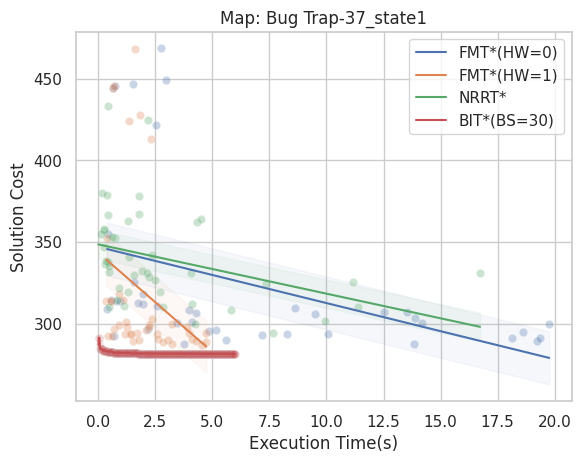
\includegraphics[scale=0.45]{scVet_Bug Trap-37_state1.png} & 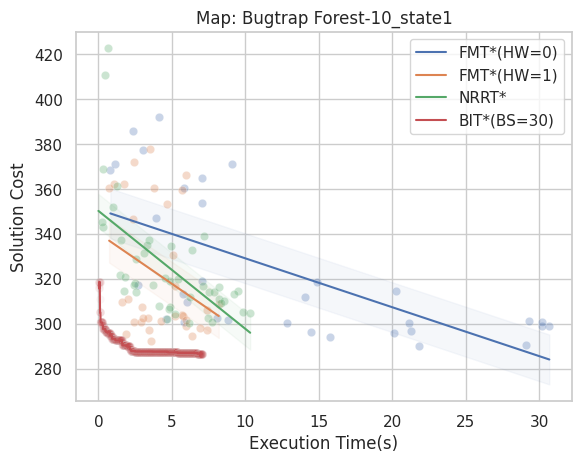
\includegraphics[scale=0.45]{scVet_Bugtrap Forest-10_state1.png}  \\
			(a) & (b)  \\[6pt]
			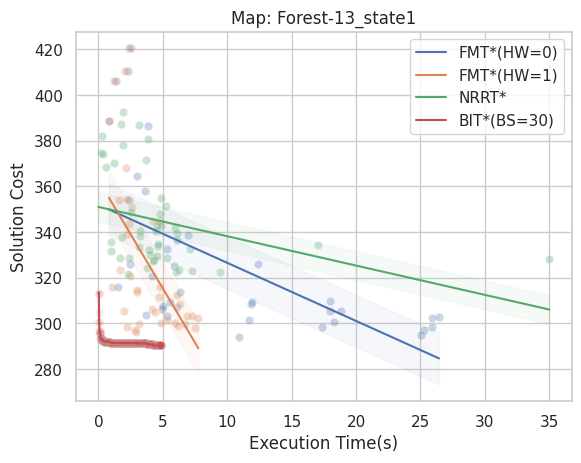
\includegraphics[scale=0.45]{scVet_Forest-13_state1.png} & 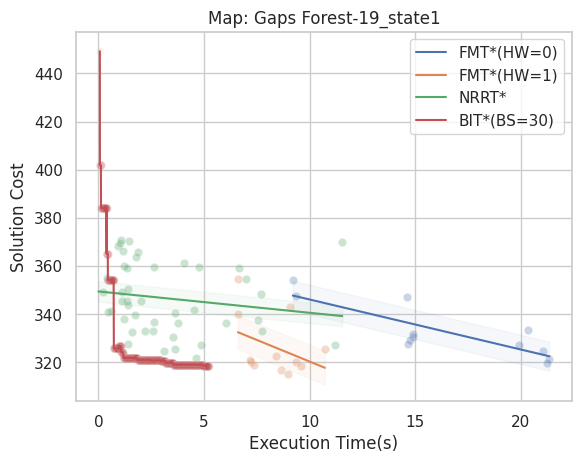
\includegraphics[scale=0.45]{scVet_Gaps Forest-19_state1.png}    \\
			(c) & (d) \\[6pt]
			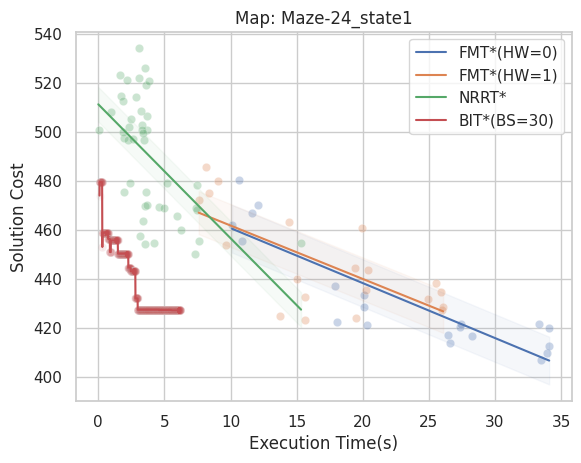
\includegraphics[scale=0.45]{scVet_Maze-24_state1.png} & 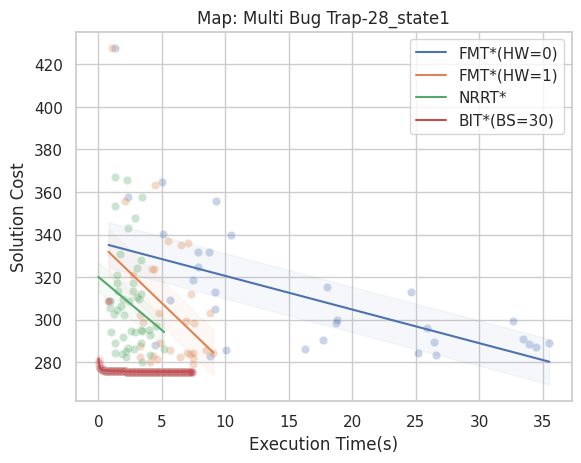
\includegraphics[scale=0.45]{scVet_Multi Bug Trap-28_state1.png}  \\
			(e) & (f)  \\[6pt]
		\end{tabular}
	}
	\caption{Comparing solution cost with runtime for FMT* without heuristics (blue), FMT* with euclidean-heuristics (weigth=1.0) (orange), BIT* with batch-size=30 (red) and NRRT* (green) in different map environments}
\end{figure}

BIT* shows the best performance in most cases with a faster convergence rate to a more optimal solution as it achieves the lowest solution cost in most cases. It is also observed that BIT* remains constant over a certain number of iterations but drops to a lower solution cost with sufficiently large number of iterations.

FMT* with euclidean-heuristics always performs much better than the standard FMT* as expected. FMT* with heuristics also seems to perform better than NRRT* in most cases. Generally, the solution cost decreases with increasing execution time.

\subsubsection{Success Rate ($\mathcal{Q}$) vs Execution Time ($\mathcal{T}$)}

\begin{figure}[H]
	\makebox[\linewidth]{
		\begin{tabular}{cc}
			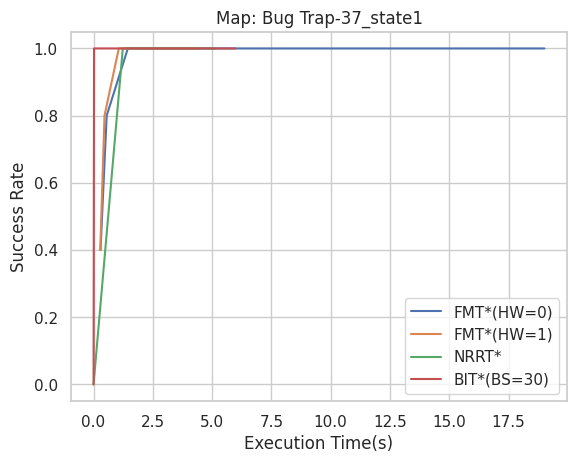
\includegraphics[scale=0.45]{srVet_Bug Trap-37_state1.png} & 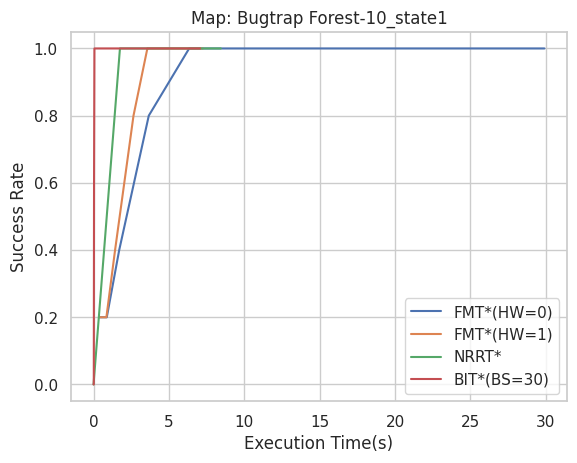
\includegraphics[scale=0.45]{srVet_Bugtrap Forest-10_state1.png}  \\
			(a) & (b)  \\[6pt]
			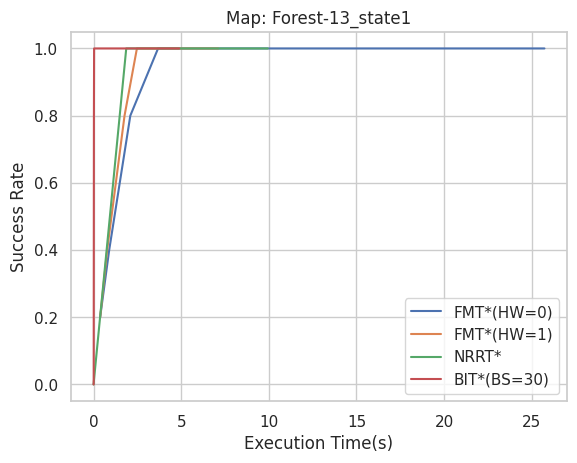
\includegraphics[scale=0.45]{srVet_Forest-13_state1.png} & 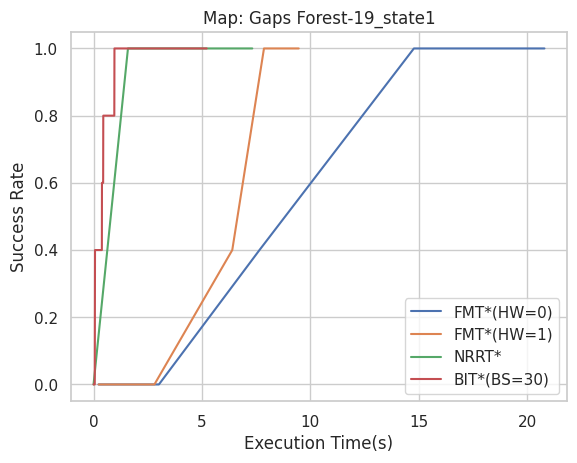
\includegraphics[scale=0.45]{srVet_Gaps Forest-19_state1.png}    \\
			(c) & (d) \\[6pt]
			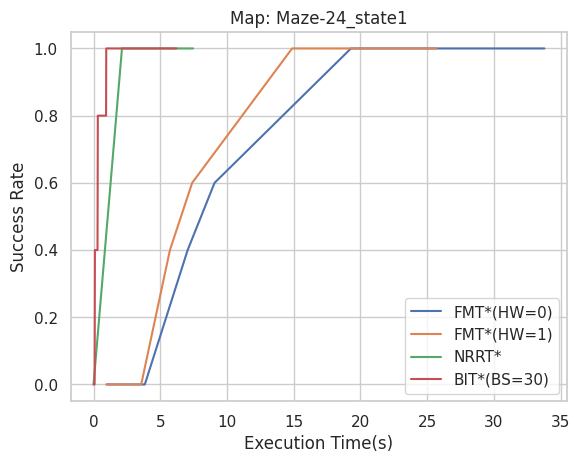
\includegraphics[scale=0.45]{srVet_Maze-24_state1.png} & 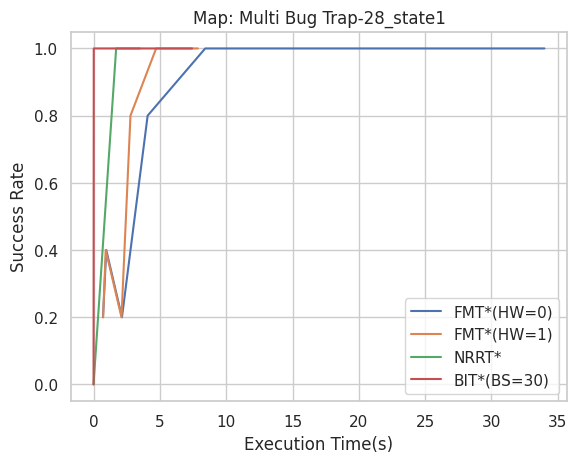
\includegraphics[scale=0.45]{srVet_Multi Bug Trap-28_state1.png}  \\
			(e) & (f)  \\[6pt]
		\end{tabular}
	}
	\caption{Comparing success rate with runtime for FMT* without heuristics (blue), FMT* with euclidean-heuristics (weigth=1.0) (orange), BIT* with batch-size=30 (red) and NRRT* (green) in different map environments}
\end{figure}

All algorithms reach $\mathcal{Q}=1.0 (\hat{\mathcal{Q}})$ within 5 seconds of execution for almost all the map environments. Only in the case of Maze and Gaps Forest, FMT* takes much longer to achieve $\hat{\mathcal{Q}}$. BIT* is the fastest in achieving $\hat{\mathcal{Q}}$ with the other algorithms showing only a marginally slower convergence in most map environments. FMT* without heuristcs is the slowest to converge in all scenarios

\subsubsection{Success Rate ($\mathcal{Q}$) vs Sample Count ($\mathcal{N}$)}

\begin{figure}[H]
	\makebox[\linewidth]{
		\begin{tabular}{cc}
			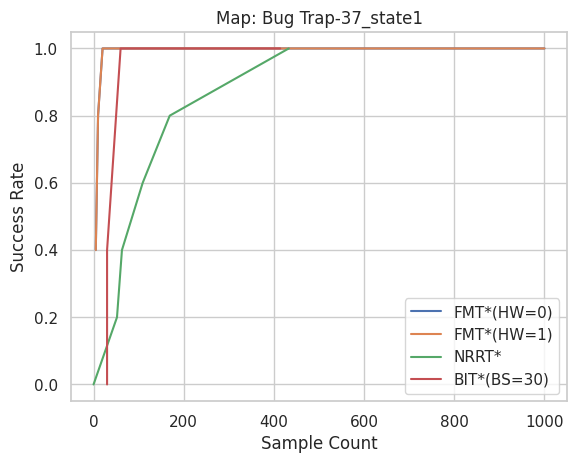
\includegraphics[scale=0.45]{srVsc_Bug Trap-37_state1.png} & 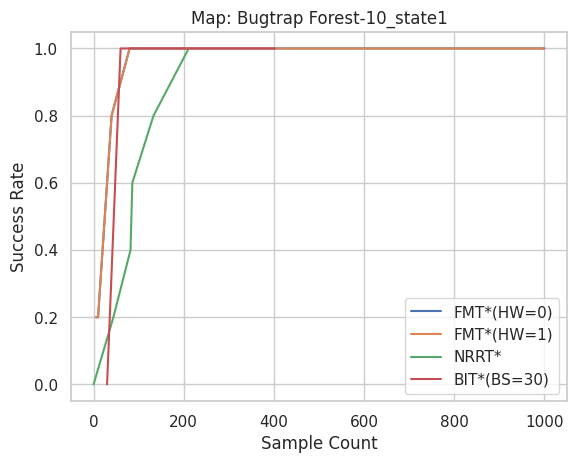
\includegraphics[scale=0.45]{srVsc_Bugtrap Forest-10_state1.png}  \\
			(a) & (b)  \\[6pt]
			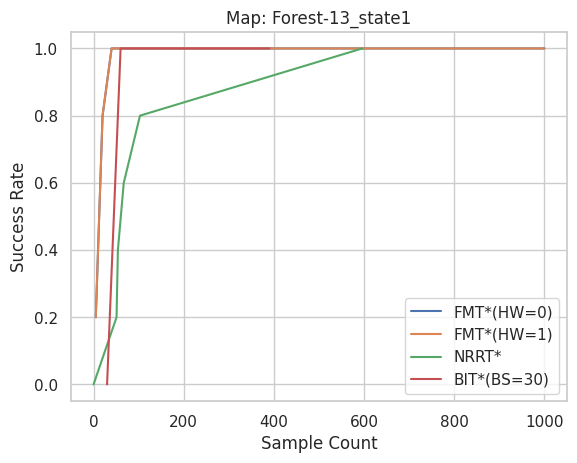
\includegraphics[scale=0.45]{srVsc_Forest-13_state1.png} & 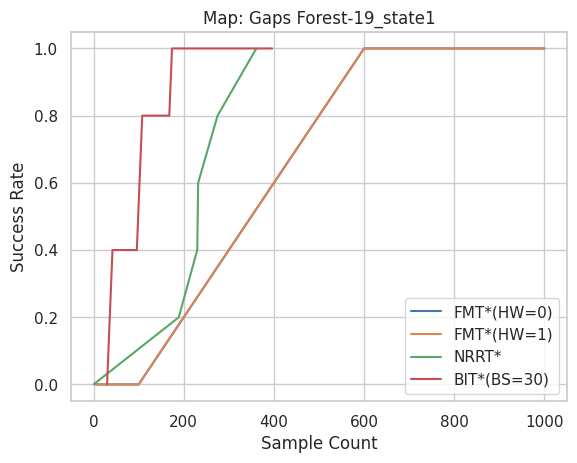
\includegraphics[scale=0.45]{srVsc_Gaps Forest-19_state1.png}    \\
			(c) & (d) \\[6pt]
			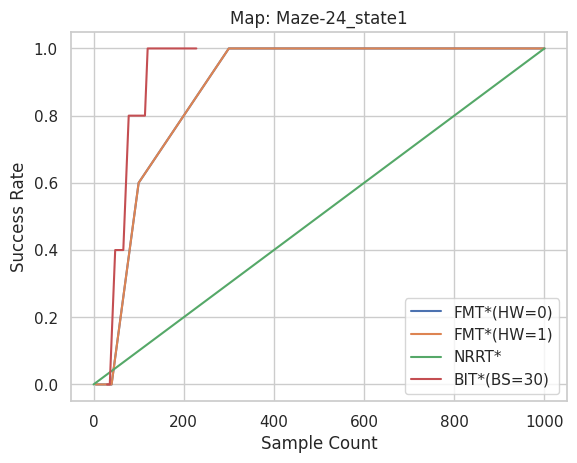
\includegraphics[scale=0.45]{srVsc_Maze-24_state1.png} & 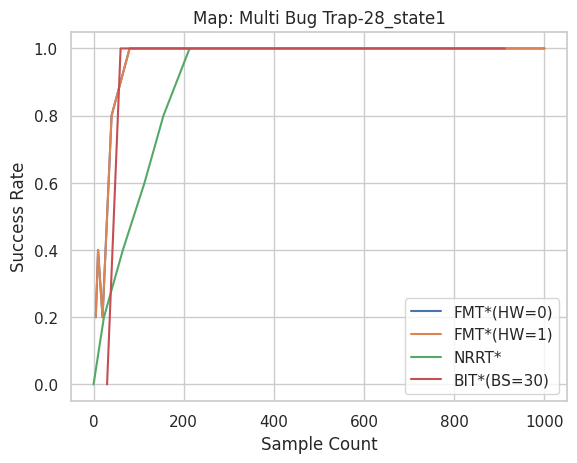
\includegraphics[scale=0.45]{srVsc_Multi Bug Trap-28_state1.png}  \\
			(e) & (f)  \\[6pt]
		\end{tabular}
	}
	\caption{Comparing success rate with sample count for FMT* without heuristics (blue), FMT* with euclidean-heuristics (weigth=1.0) (orange), BIT* with batch-size=30 (red) and NRRT* (green) in different map environments}
\end{figure}

For BugTrap and Forest (simple environments), FMT* requires a relatively smaller sample count ($\sim 80$) to achieve $\hat{\mathcal{Q}}$. However, for more complex enviroments such as BugTrap-Forest, Gaps-Forest, Maze and Multi-BugTrap, BIT* achieves $\hat{\mathcal{Q}}$ most efficiently. A noteworthy point about BIT* is that it is able to achieve $\hat{\mathcal{Q}}$ with almost the same sample count ($\sim 100$) in all map environments. NRRT* seems to require a relatively larger sample count to achieve $\hat{\mathcal{Q}}$ in most map environments.

\subsubsection{Sample Count ($\mathcal{N}$) vs Number of collision checks ($\mathcal{C}$)}

\begin{figure}[H]
	\makebox[\linewidth]{
		\begin{tabular}{cc}
			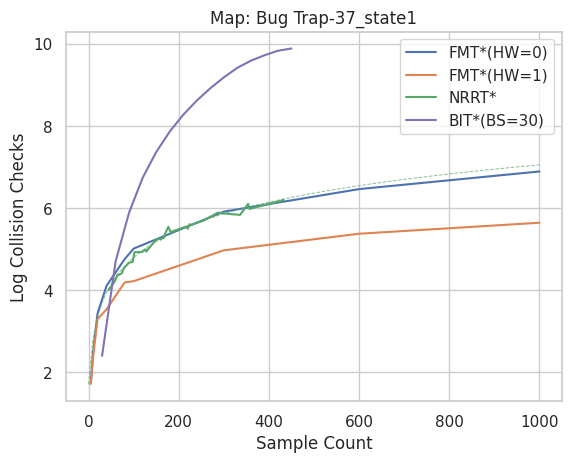
\includegraphics[scale=0.45]{scVcc_Bug Trap-37_state1.png} & 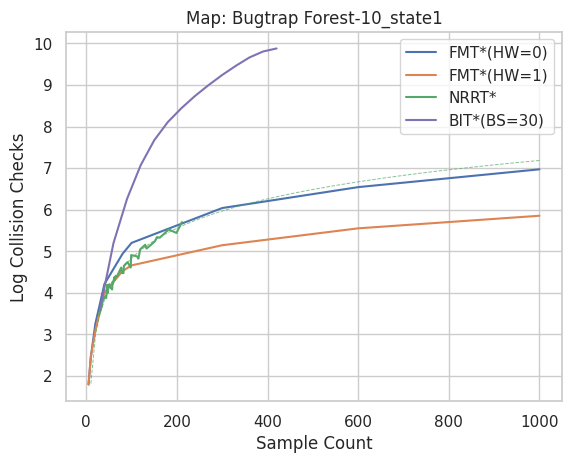
\includegraphics[scale=0.45]{scVcc_Bugtrap Forest-10_state1.png}  \\
			(a) & (b)  \\[6pt]
			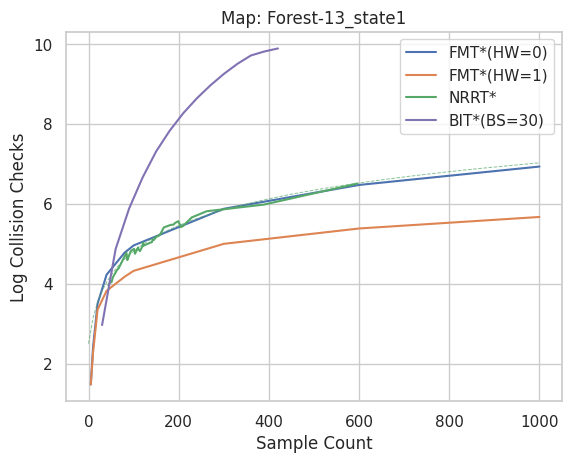
\includegraphics[scale=0.45]{scVcc_Forest-13_state1.png} & 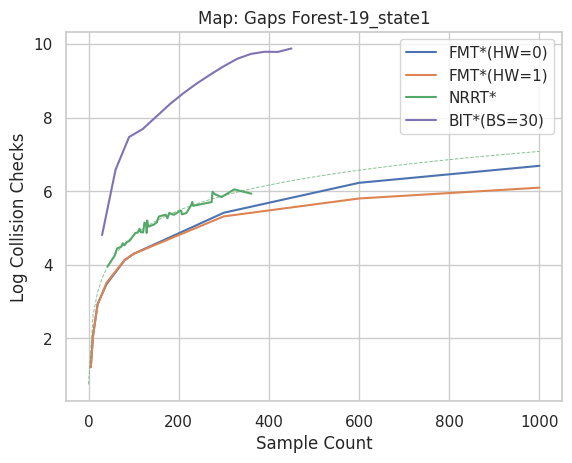
\includegraphics[scale=0.45]{scVcc_Gaps Forest-19_state1.png}    \\
			(c) & (d) \\[6pt]
			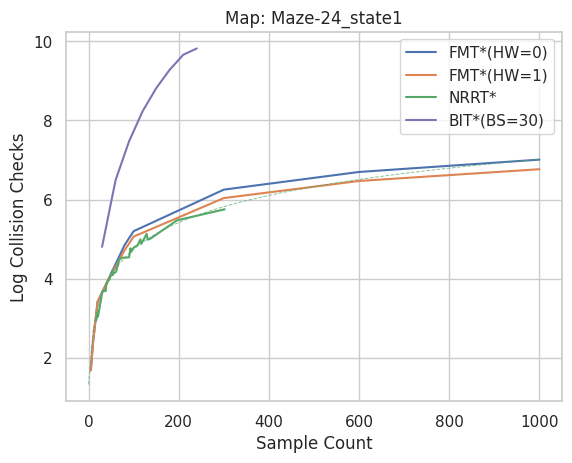
\includegraphics[scale=0.45]{scVcc_Maze-24_state1.png} & 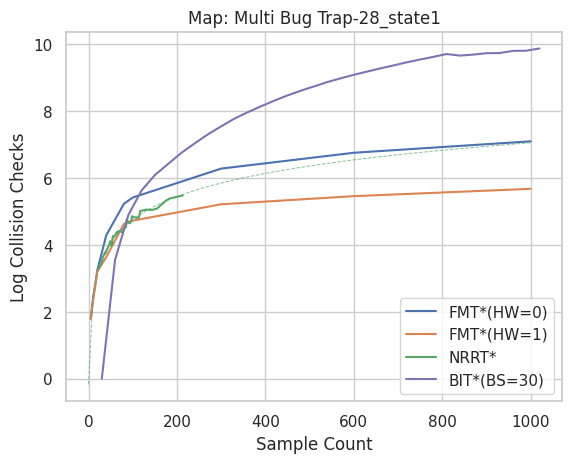
\includegraphics[scale=0.45]{scVcc_Multi Bug Trap-28_state1.png}  \\
			(e) & (f)  \\[6pt]
		\end{tabular}
	}
	\caption{Comparing sample count with number of collision checks made by FMT* without heuristics (blue), FMT* with euclidean-heuristics (weigth=1.0) (orange), BIT* with batch-size=30 (red) and NRRT* (green) in different map environments}
\end{figure}

In this analysis, it is clearly observed that FMT* performs significantly fewer collision checks compared to BIT*. FMT* with euclidean-heuristics performs the least number of collision checks. Maximum number of collision checks performed by FMT* is for the maze environment. This trend describes the "lazy collision checking" behavior of FMT* which is what makes it perform better in high dimensional environments. 

\subsection{Qualitative Analysis: Generated Paths}

\textbf{\underline{FMT*:}}

FMT* progressively improves on the optimality of the path found as the sample count is increased. This can be observed from the paths generated by FMT* for the Maze environment with increasing sample count as shown in Fig. \ref{fmt:nsamples}

\begin{figure}[H]
	\makebox[\linewidth]{
		\begin{tabular}{ccc}
			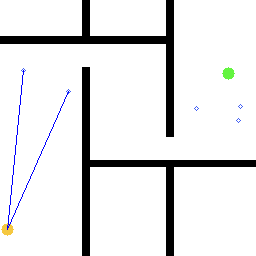
\includegraphics[scale=0.3]{fmt_paths/n_samples/0.png} & 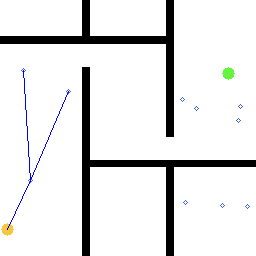
\includegraphics[scale=0.3]{fmt_paths/n_samples/1.png} & 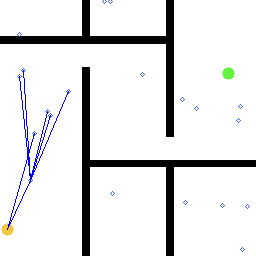
\includegraphics[scale=0.3]{fmt_paths/n_samples/2.png}\\
			(a) & (b) & (c)\\[6pt]
			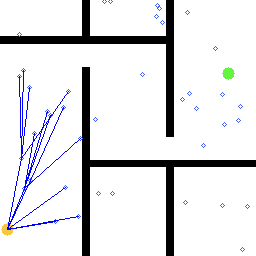
\includegraphics[scale=0.3]{fmt_paths/n_samples/3.png} & 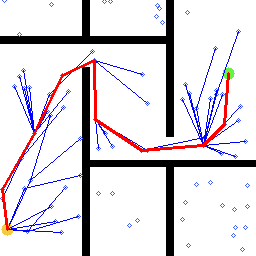
\includegraphics[scale=0.3]{fmt_paths/n_samples/4.png} & 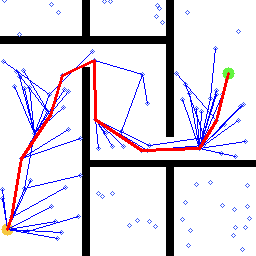
\includegraphics[scale=0.3]{fmt_paths/n_samples/5.png}\\
			(d) & (e) & (f)\\[6pt]
			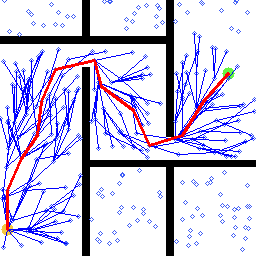
\includegraphics[scale=0.3]{fmt_paths/n_samples/6.png} & 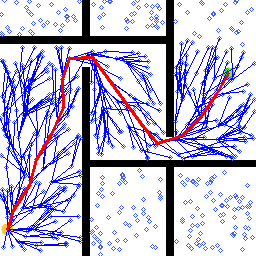
\includegraphics[scale=0.3]{fmt_paths/n_samples/7.png} & 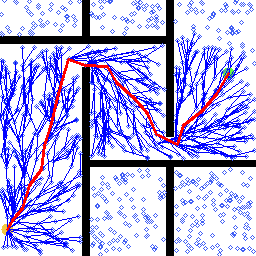
\includegraphics[scale=0.3]{fmt_paths/n_samples/8.png}\\
			(g) & (h) & (i)\\[6pt]
		\end{tabular}
	}
	\caption{Paths generated by FMT* (without heuristics) for the maze environment with increasing sample count: (a)-5, (b)-10, (c)-20, (d)-40, (e)-80, (f)-100, (g)-300, (h)-600, (i)-1000. Red line indicates the final path generated by the algorithm}
	\label{fmt:nsamples}
\end{figure}

As the sample count increases, the algorithm is able to avoid unnecessary turns to generate a path with longer linear-subpaths thus minimizing the cost.

An additional set of simulations were performed for FMT* specifically which incorporates euclidean-heuristics (as described in \ref{met:fmt}). The paths generated by each FMT* algorithm on the Forest map is described in Fig.

\begin{figure}[H]
	\makebox[\linewidth]{
		\begin{tabular}{cc}
			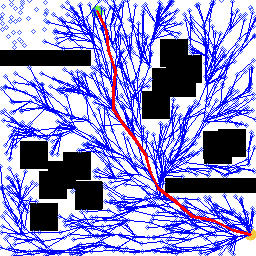
\includegraphics[scale=0.4]{fmt_paths/heuristics/0.png} & 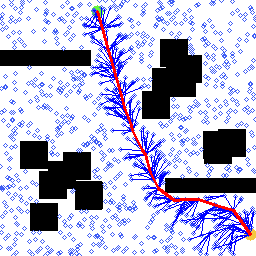
\includegraphics[scale=0.4]{fmt_paths/heuristics/1.png} \\
			(a) & (b)\\[6pt]
		\end{tabular}
	}
	\caption{Paths generated by FMT* on the Forest map: (a)- without heuristics and (b) - with euclidean-heuristics (weight=1.0). Red line indicates the final path generated by the algorithm. Blue lines indicate the nodes visited by the algorithm}
	\label{fmt:nsamples}
\end{figure}

FMT* with euclidean-heuristics visits fewer nodes while searching for a path and is thus able to converge faster. Since we use euclidean-heuristics with a euclidean cost-to-come to pick the next node in the tree, FMT* with heuristics is able to generate a more optimal path than the standard FMT* algorithm.

\textbf{\underline{BIT*:}}

//ADD RELEVANT PATH PLOTS - Jazib//

\textbf{\underline{NRRT*:}}

//ADD RELEVANT PATH PLOTS - Jimmy//

\subsection{Analyzing edge-cases: State Specific Configurations}

\subsubsection{Straight line paths}

In one of the simulations run on the Gaps-Forest map, the path from {\varfont start} to {\varfont goal} was a straight line with no obstacles along this line. In this section, we qualitatively compare the paths generated by each algorithm in such a scenario

\textbf{\underline{FMT*:}}

\begin{figure}[H]
	\makebox[\linewidth]{
		\begin{tabular}{cc}
			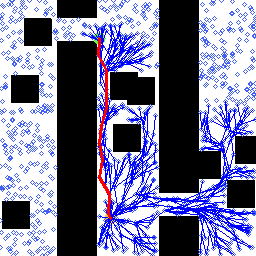
\includegraphics[scale=0.4]{fmt_paths/straight_line/0.png} & 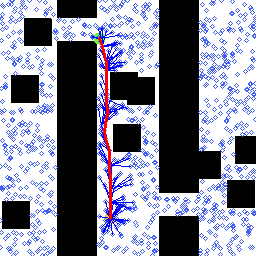
\includegraphics[scale=0.4]{fmt_paths/straight_line/1.png} \\
			(a) & (b)\\[6pt]
		\end{tabular}
	}
	\caption{Paths generated by FMT* on the Gaps-Forest map: (a)- without heuristics and (b) - with euclidean-heuristics (weight=1.0). Red line indicates the final path generated by the algorithm. Blue lines indicate the nodes visited by the algorithm}
	\label{fmt:nsamples}
\end{figure}

\textbf{\underline{BIT*:}}

\begin{figure}[H]
	\makebox[\linewidth]{
		\begin{tabular}{c}
			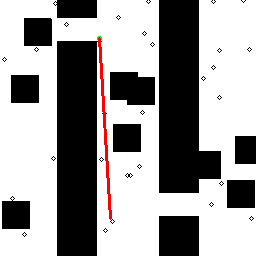
\includegraphics[scale=0.4]{bit_paths/straight_line/0.png} \\
		\end{tabular}
	}
	\caption{Path generated by BIT* on the Gaps-Forest map. Red line indicates the final path generated by the algorithm.}
	\label{fmt:nsamples}
\end{figure}

\textbf{\underline{NRRT*:}}

\begin{figure}[H]
	\makebox[\linewidth]{
		\begin{tabular}{c}
			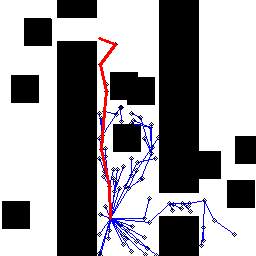
\includegraphics[scale=0.4]{nrrt_paths/straight_line/0.png} \\
		\end{tabular}
	}
	\caption{Path generated by NRRT* on the Gaps-Forest map. Red line indicates the final path generated by the algorithm.}
	\label{fmt:nsamples}
\end{figure}

\subsubsection{Unreachable goals}

Often times, there are cases where the goal is unreachable from the start location on the map. We outline one such case that we encountered during our simulations for the Maze environment where the goal was entirely enclosed by obstacles. In such situations, it is important to evaluate how fast can the algorithm can report "no-solution". This can be evaluated using two metrics: Mean execution time per sample count and Mean number of collision check per sample count. We compute and report these metrics for the three algorithms in Table. \ref{un:mets}.

\begin{table}[H]
	\caption{Running FMT*, BIT* and NRRT* on a map with an unreachable goal}
	\makebox[\linewidth]{
		\begin{tabular}{|c|c|c|}
			\hline
			Alg. & \begin{tabular}{@{}c@{}}Mean execution time \\ per sample count\end{tabular} & \begin{tabular}{@{}c@{}}Mean no. collision checks \\ per sample count\end{tabular}\\
			\hline
			FMT* & 0.082 & 1.48\\
			\hline
			\begin{tabular}{@{}c@{}}FMT* \\ (with heuristics)\end{tabular} & 0.080 & 1.48\\
			\hline
			BIT* & 0.021 & 63.25\\
			\hline
			NRRT* & 0.026 & 1.19\\
			\hline
		\end{tabular}
		}
	\label{un:mets}
\end{table}


\section{Limitations}
Something...

\section{Conclusion}
We presented a comparison...

\subsection*{Acknowledgements}

    
\clearpage

\bibliography{report}
%\bibliographystyle{apj}

\clearpage

\section*{Appendix A: Maps}
    
    Map images
    
\clearpage

\section*{Appendix B: Plot type 1}
    
    Plots
    
\clearpage

\section*{Appendix C: Plot type 2}
    
    Plots

\clearpage

\section*{Appendix D: Group Contributions}
    
    Jazib Ahmad contributed...

\clearpage

\end{document}

%===============================================================================

% The maximum paper length is 8 pages excluding references and acknowledgements, and 10 pages including references and acknowledgements

%===============================================================================